\chapter{Developing Physics-based Approaches towards PMP Estimation: Supplemental Materials}

This appendix includes the supplemental materials for chapter \ref{ch:JHM}. As the time of writing the dissertation, these materials have been under review for the \textit{Journal of Hydrometeorology}.

\bigbreak

\noindent
\hangafter=1
\setlength{\hangindent}{2em}
Chen, X. and Hossain, F., Understanding Model-based Probable Maximum Precipitation Estimation as a Function of Location and Season from Atmospheric Reanalysis. \textit{Journal of Hydrometeorology} (under review).

\vspace{10mm}

\noindent

\section{Figures}

\begin{figure}[htbp]
	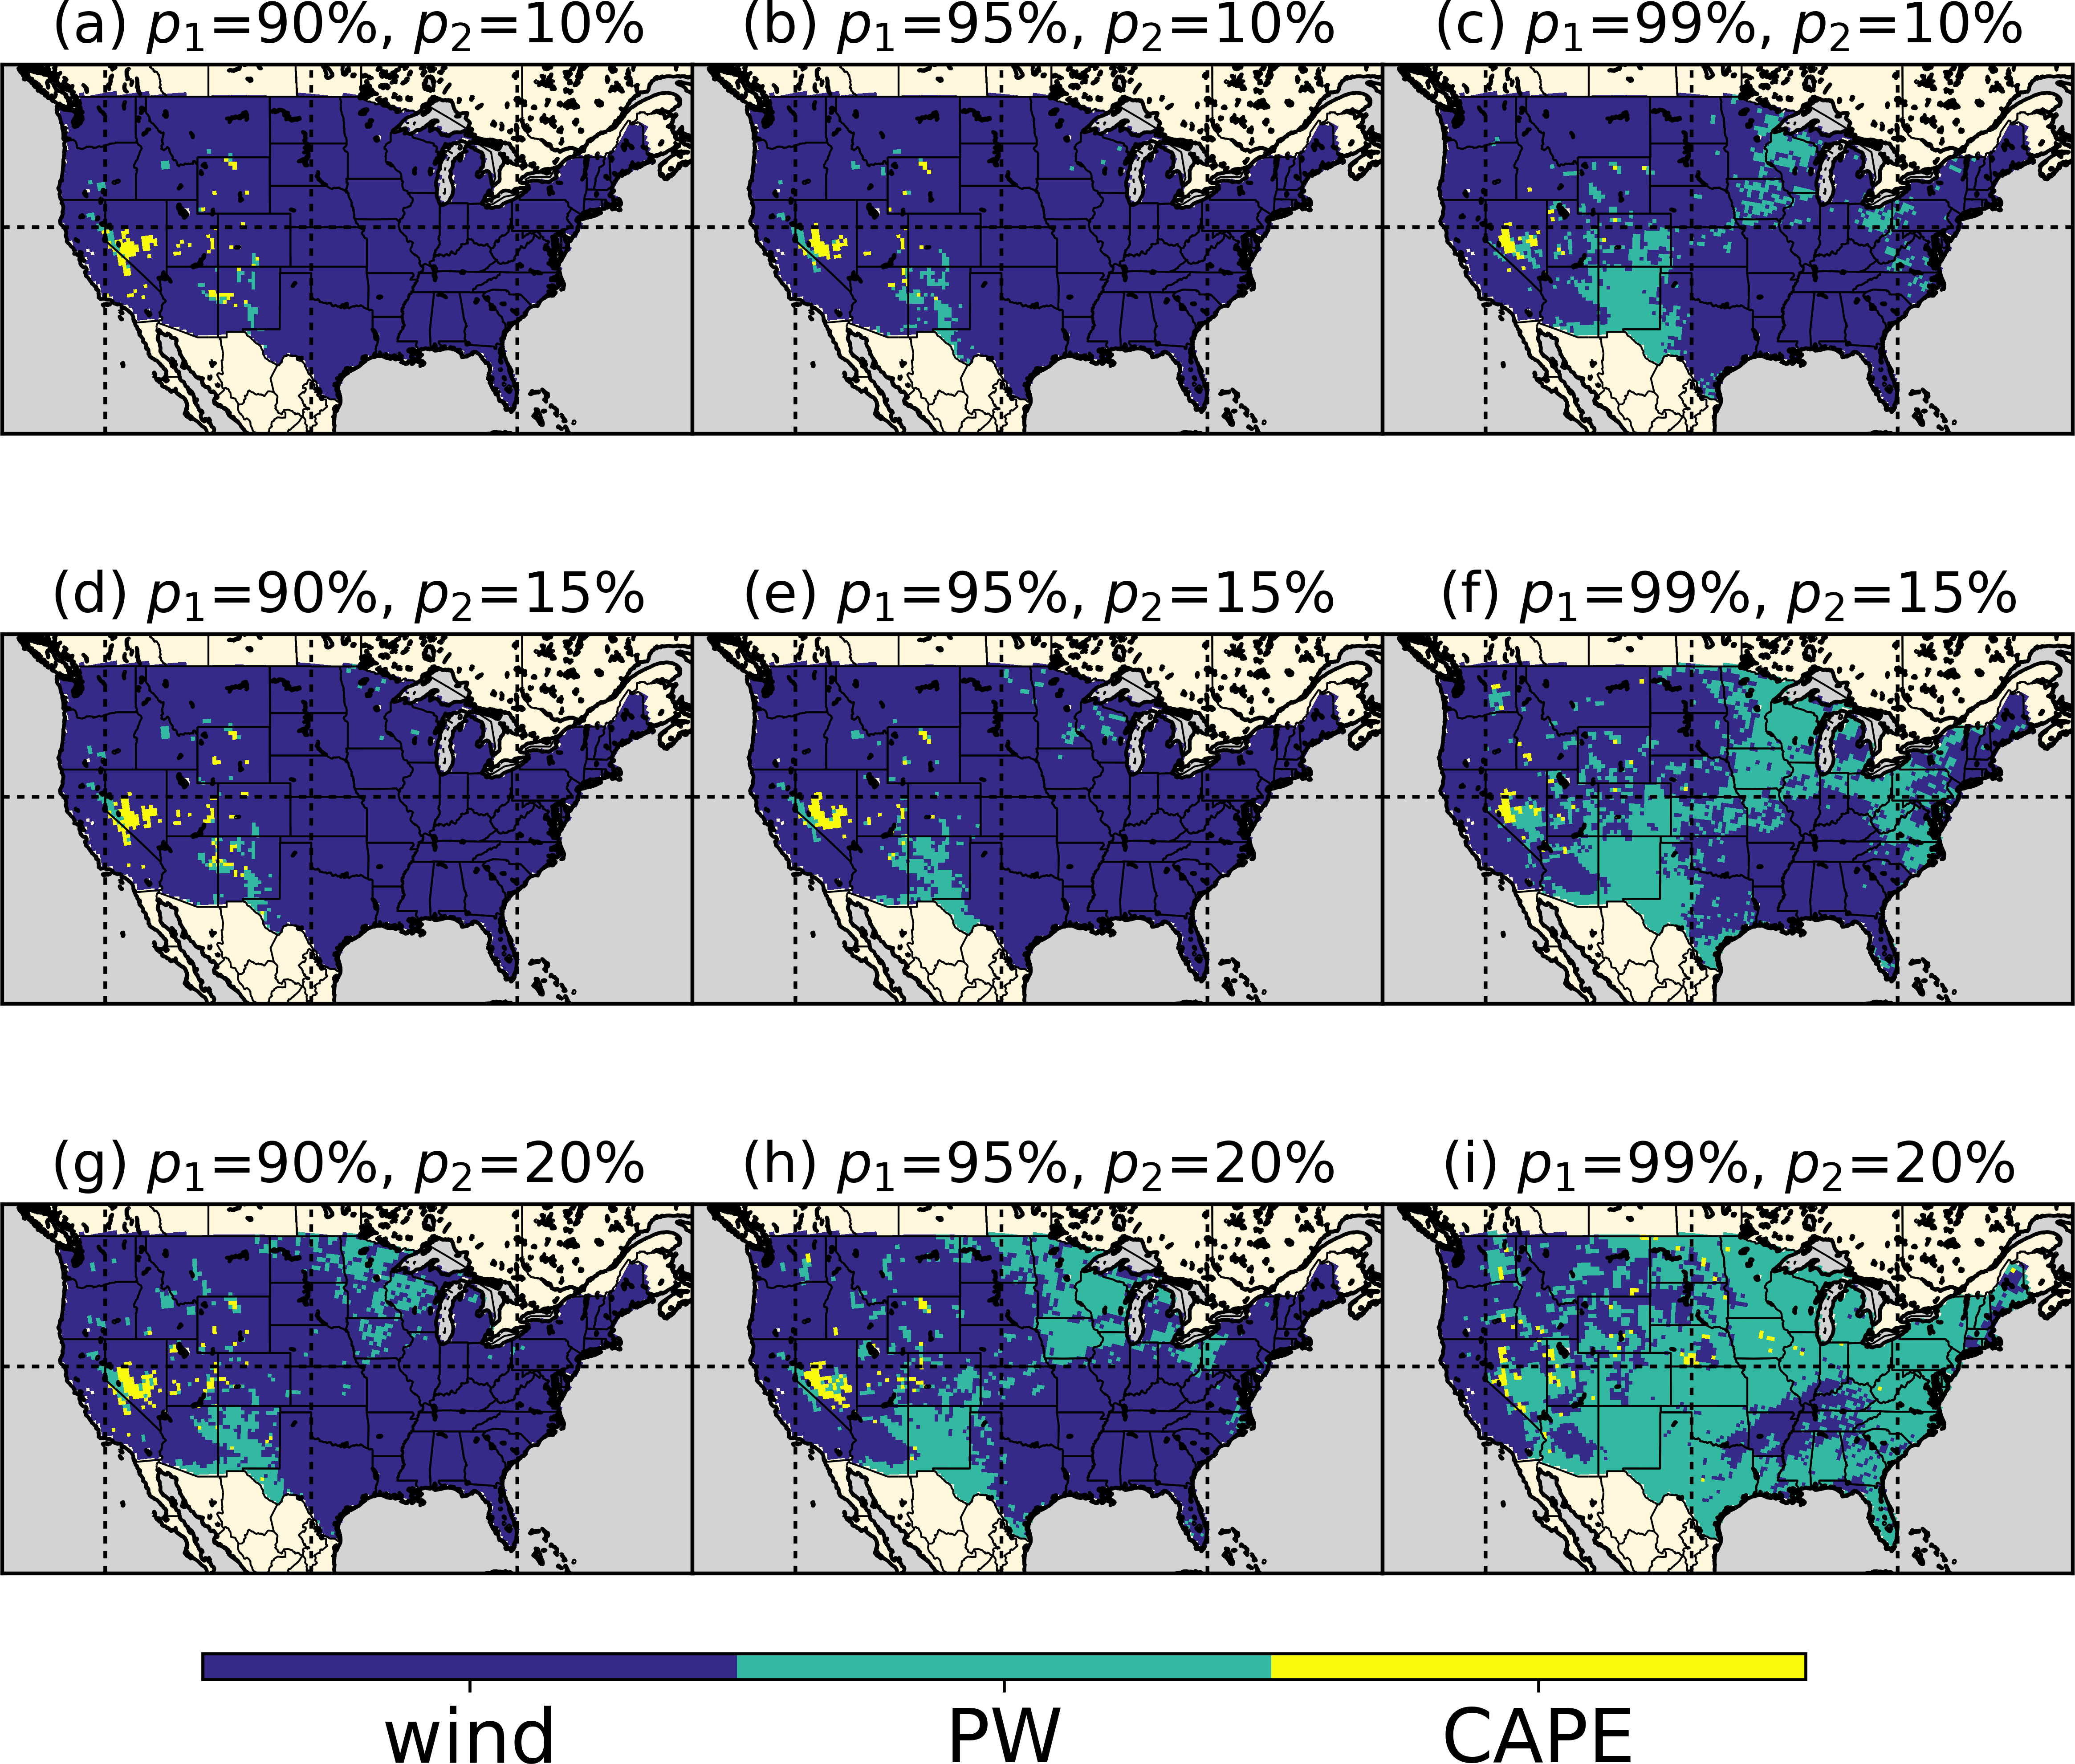
\includegraphics[width=16cm]{pics/ch4/figS1.png}
	\caption{Robustness check of the derived map in figure \ref{fig:4-5}a. Here the two parameters are perturbed within a range ($90\%\scriptsize{\sim}99\%$ for p1, $10\%\scriptsize{\sim}20\%$ for p2), and the derived maps share a similar pattern as figure \ref{fig:4-5}a.}
	\label{fig:4-S1}
\end{figure}

\begin{figure}[htbp]
	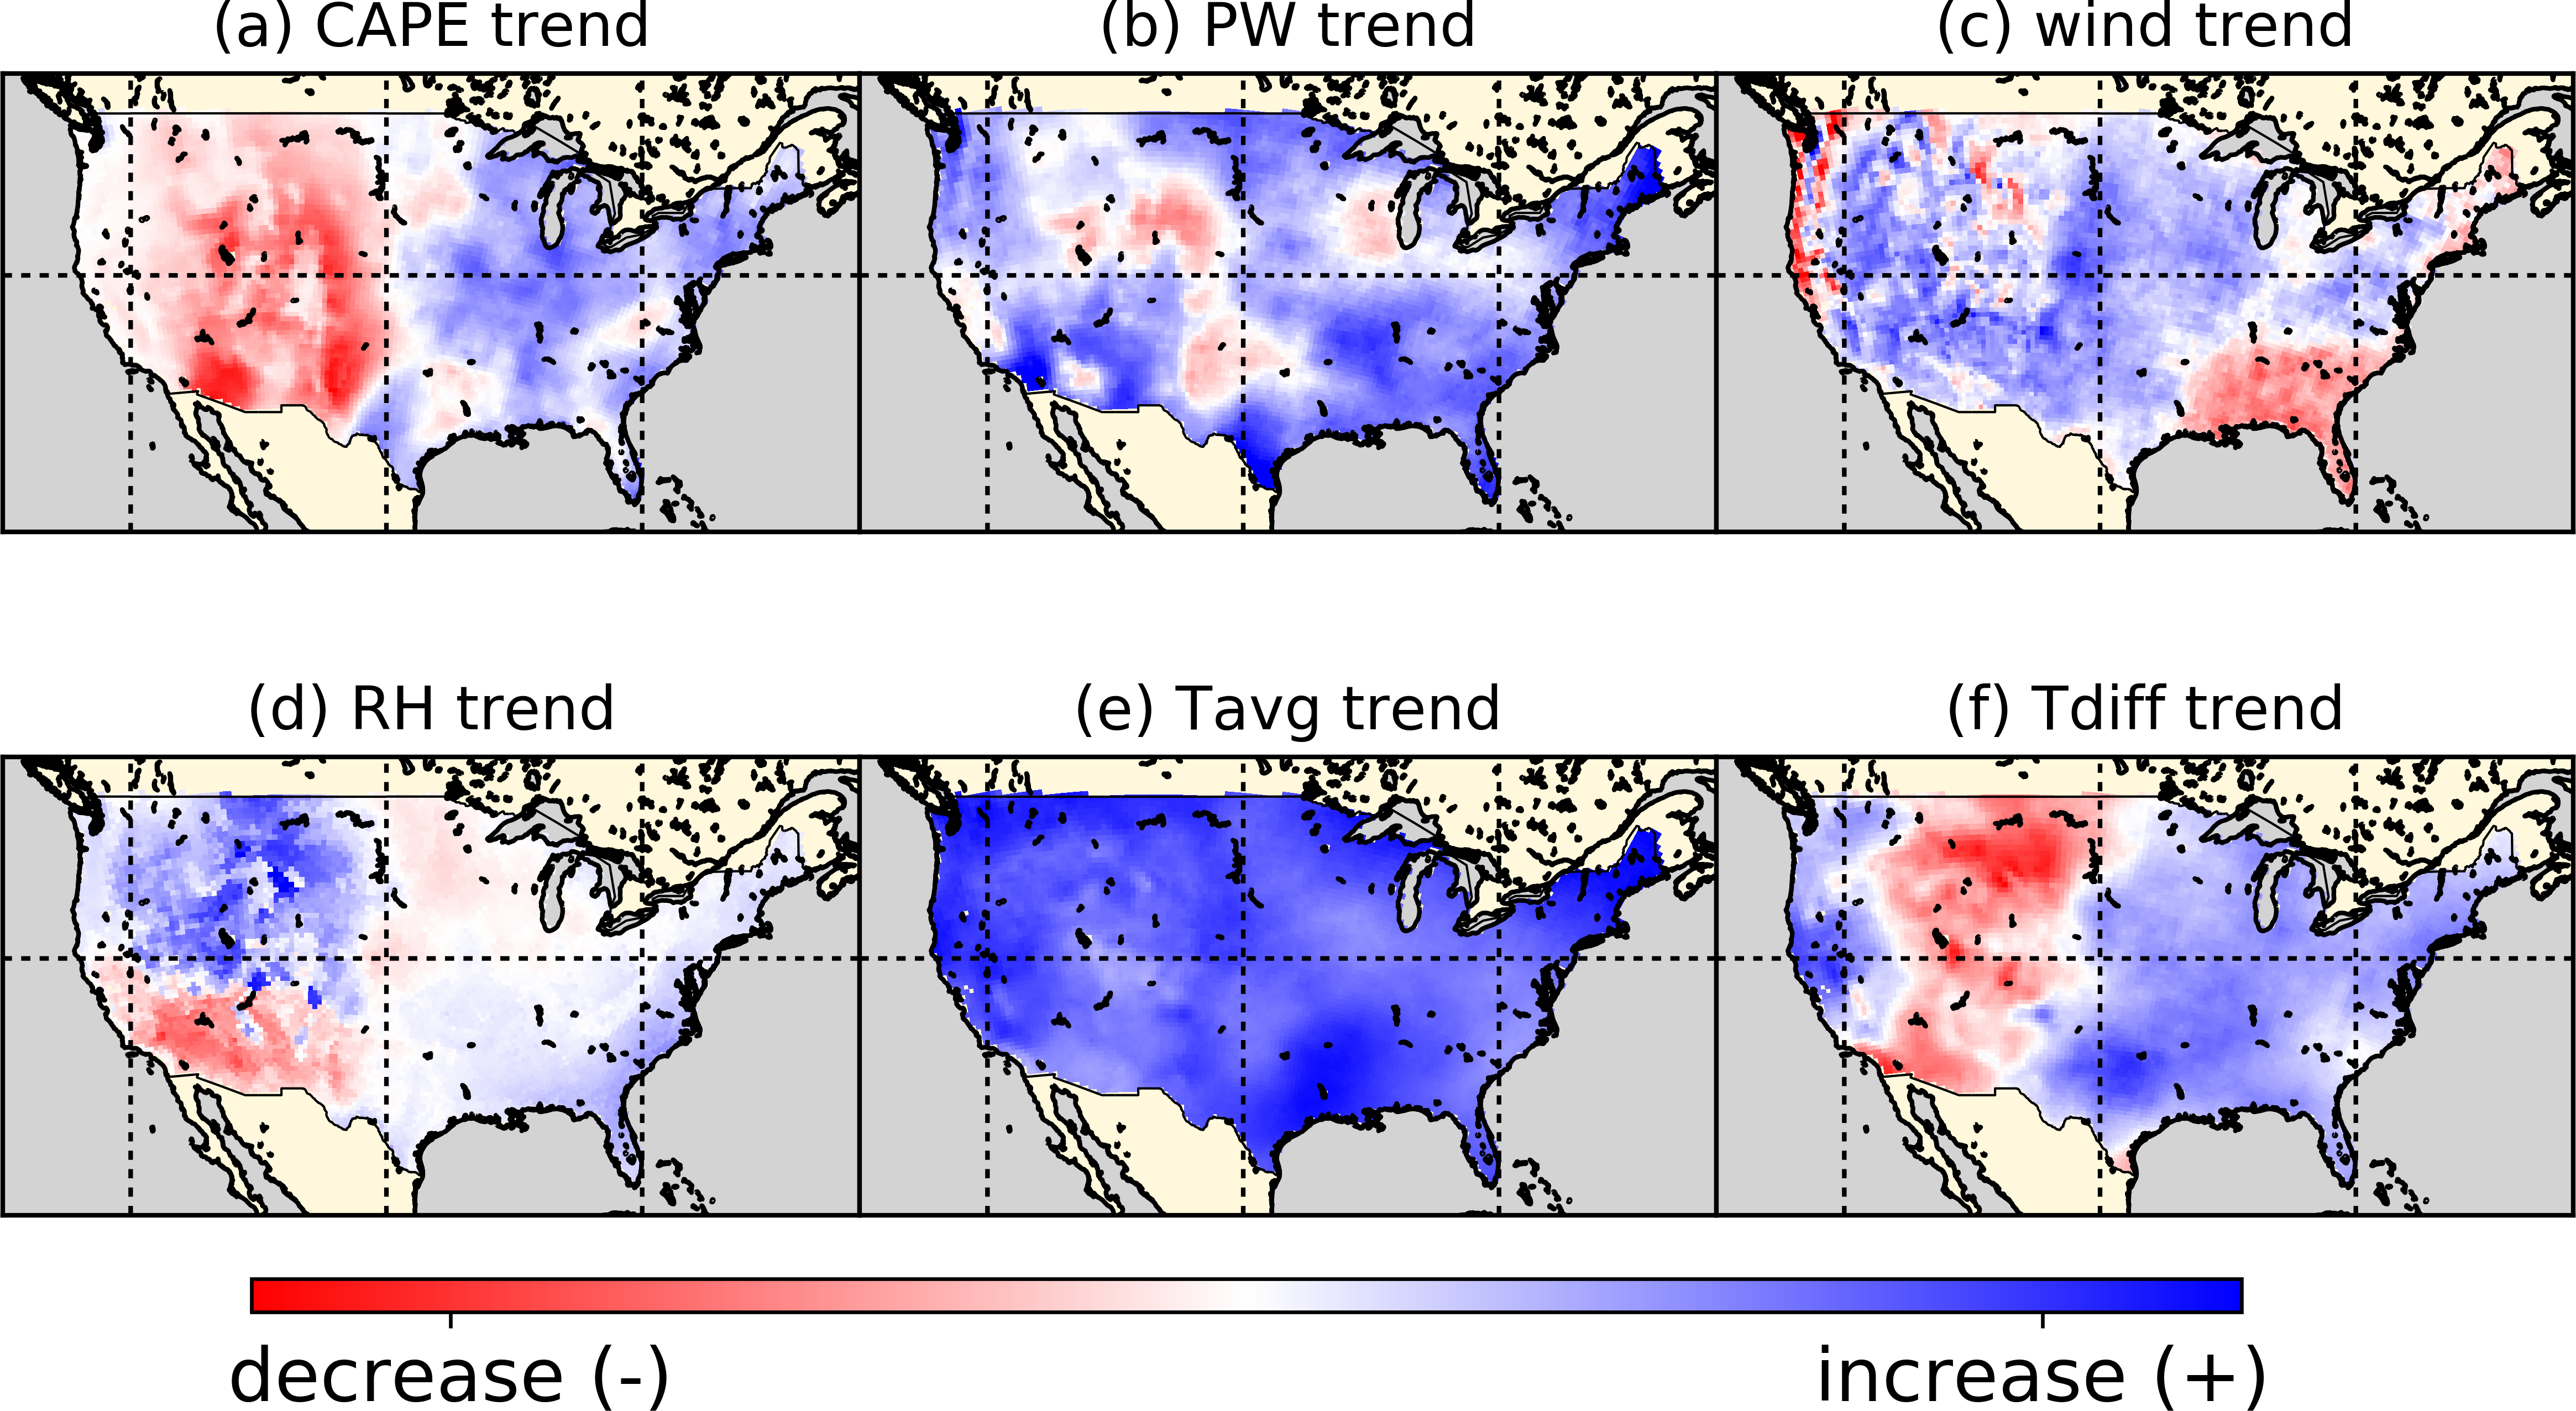
\includegraphics[width=\linewidth]{pics/ch4/figS2.png}
	\caption{Trends of meteorological factors analyzed in this study during 1979-2015. For each year, the 20-year ARI value is calculated for each factor. Then the series between 1979 and 2015 are used to calculate these trends.}
	\label{fig:4-S2}
\end{figure}

\begin{figure}[htbp]
	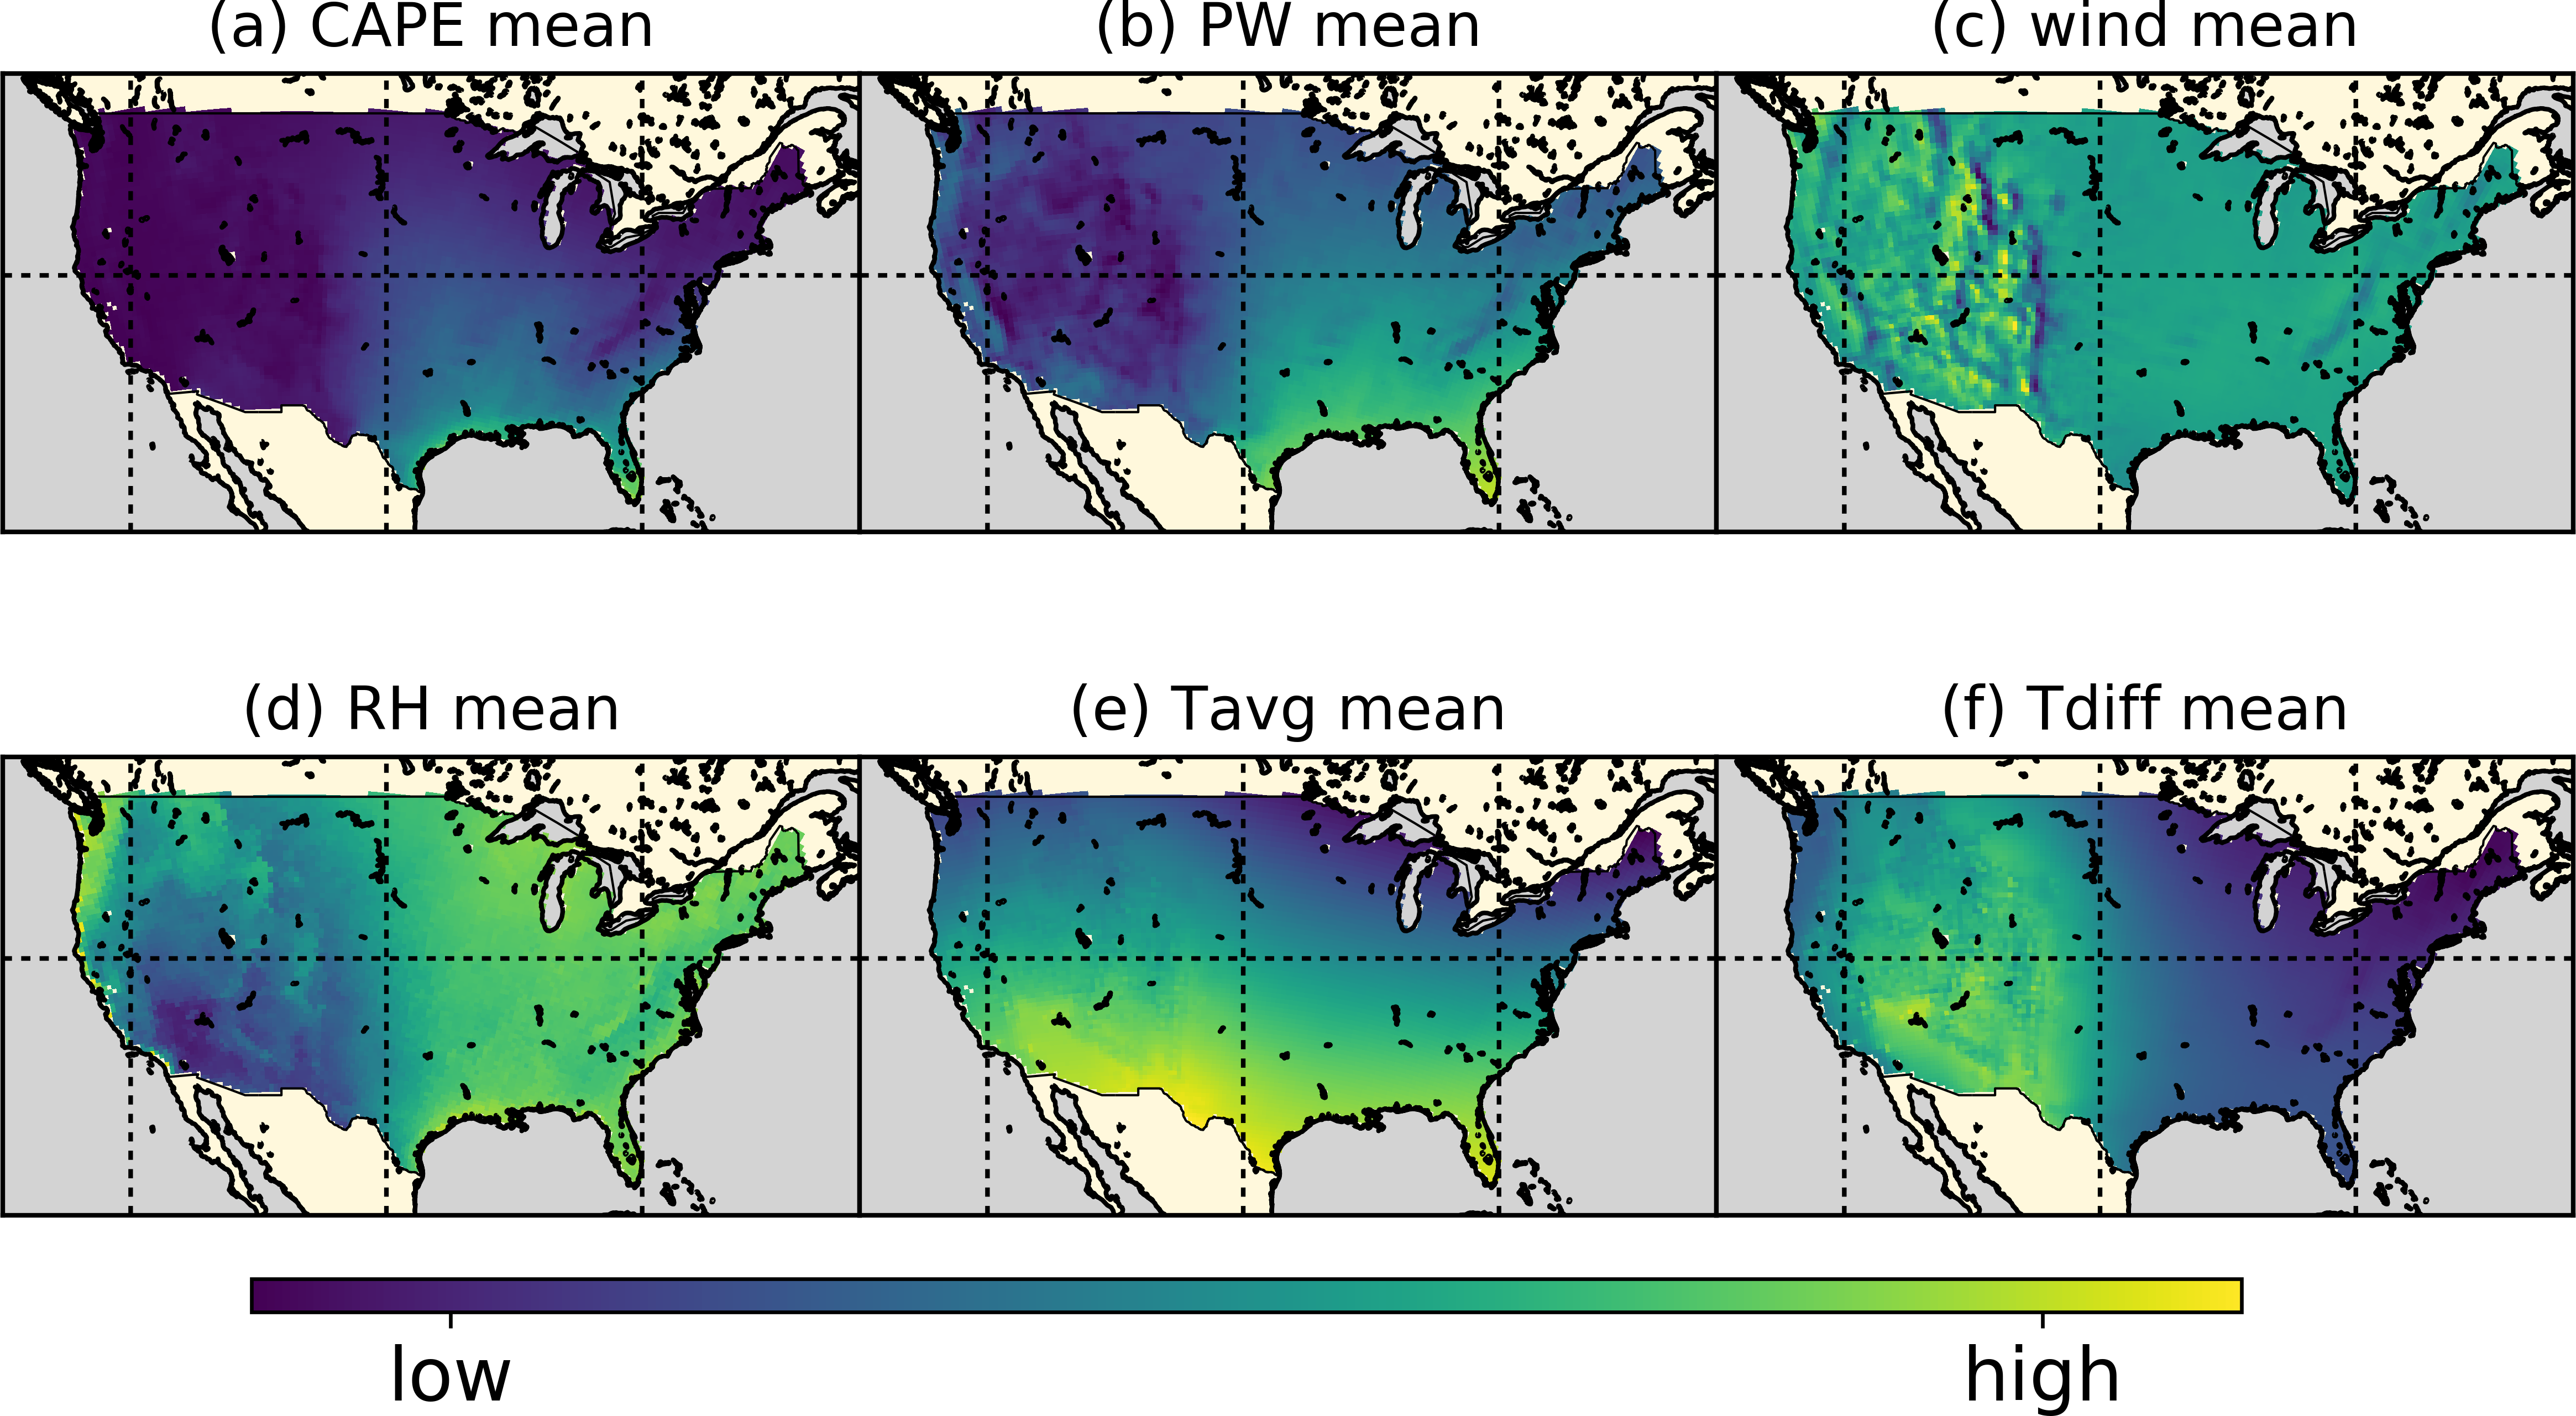
\includegraphics[width=\linewidth]{pics/ch4/figS3.png}
	\caption{Climatology of the meteorological factors analyzed in this study during 1979-2015.}
	\label{fig:4-S3}
\end{figure}

\begin{figure}[htbp]
	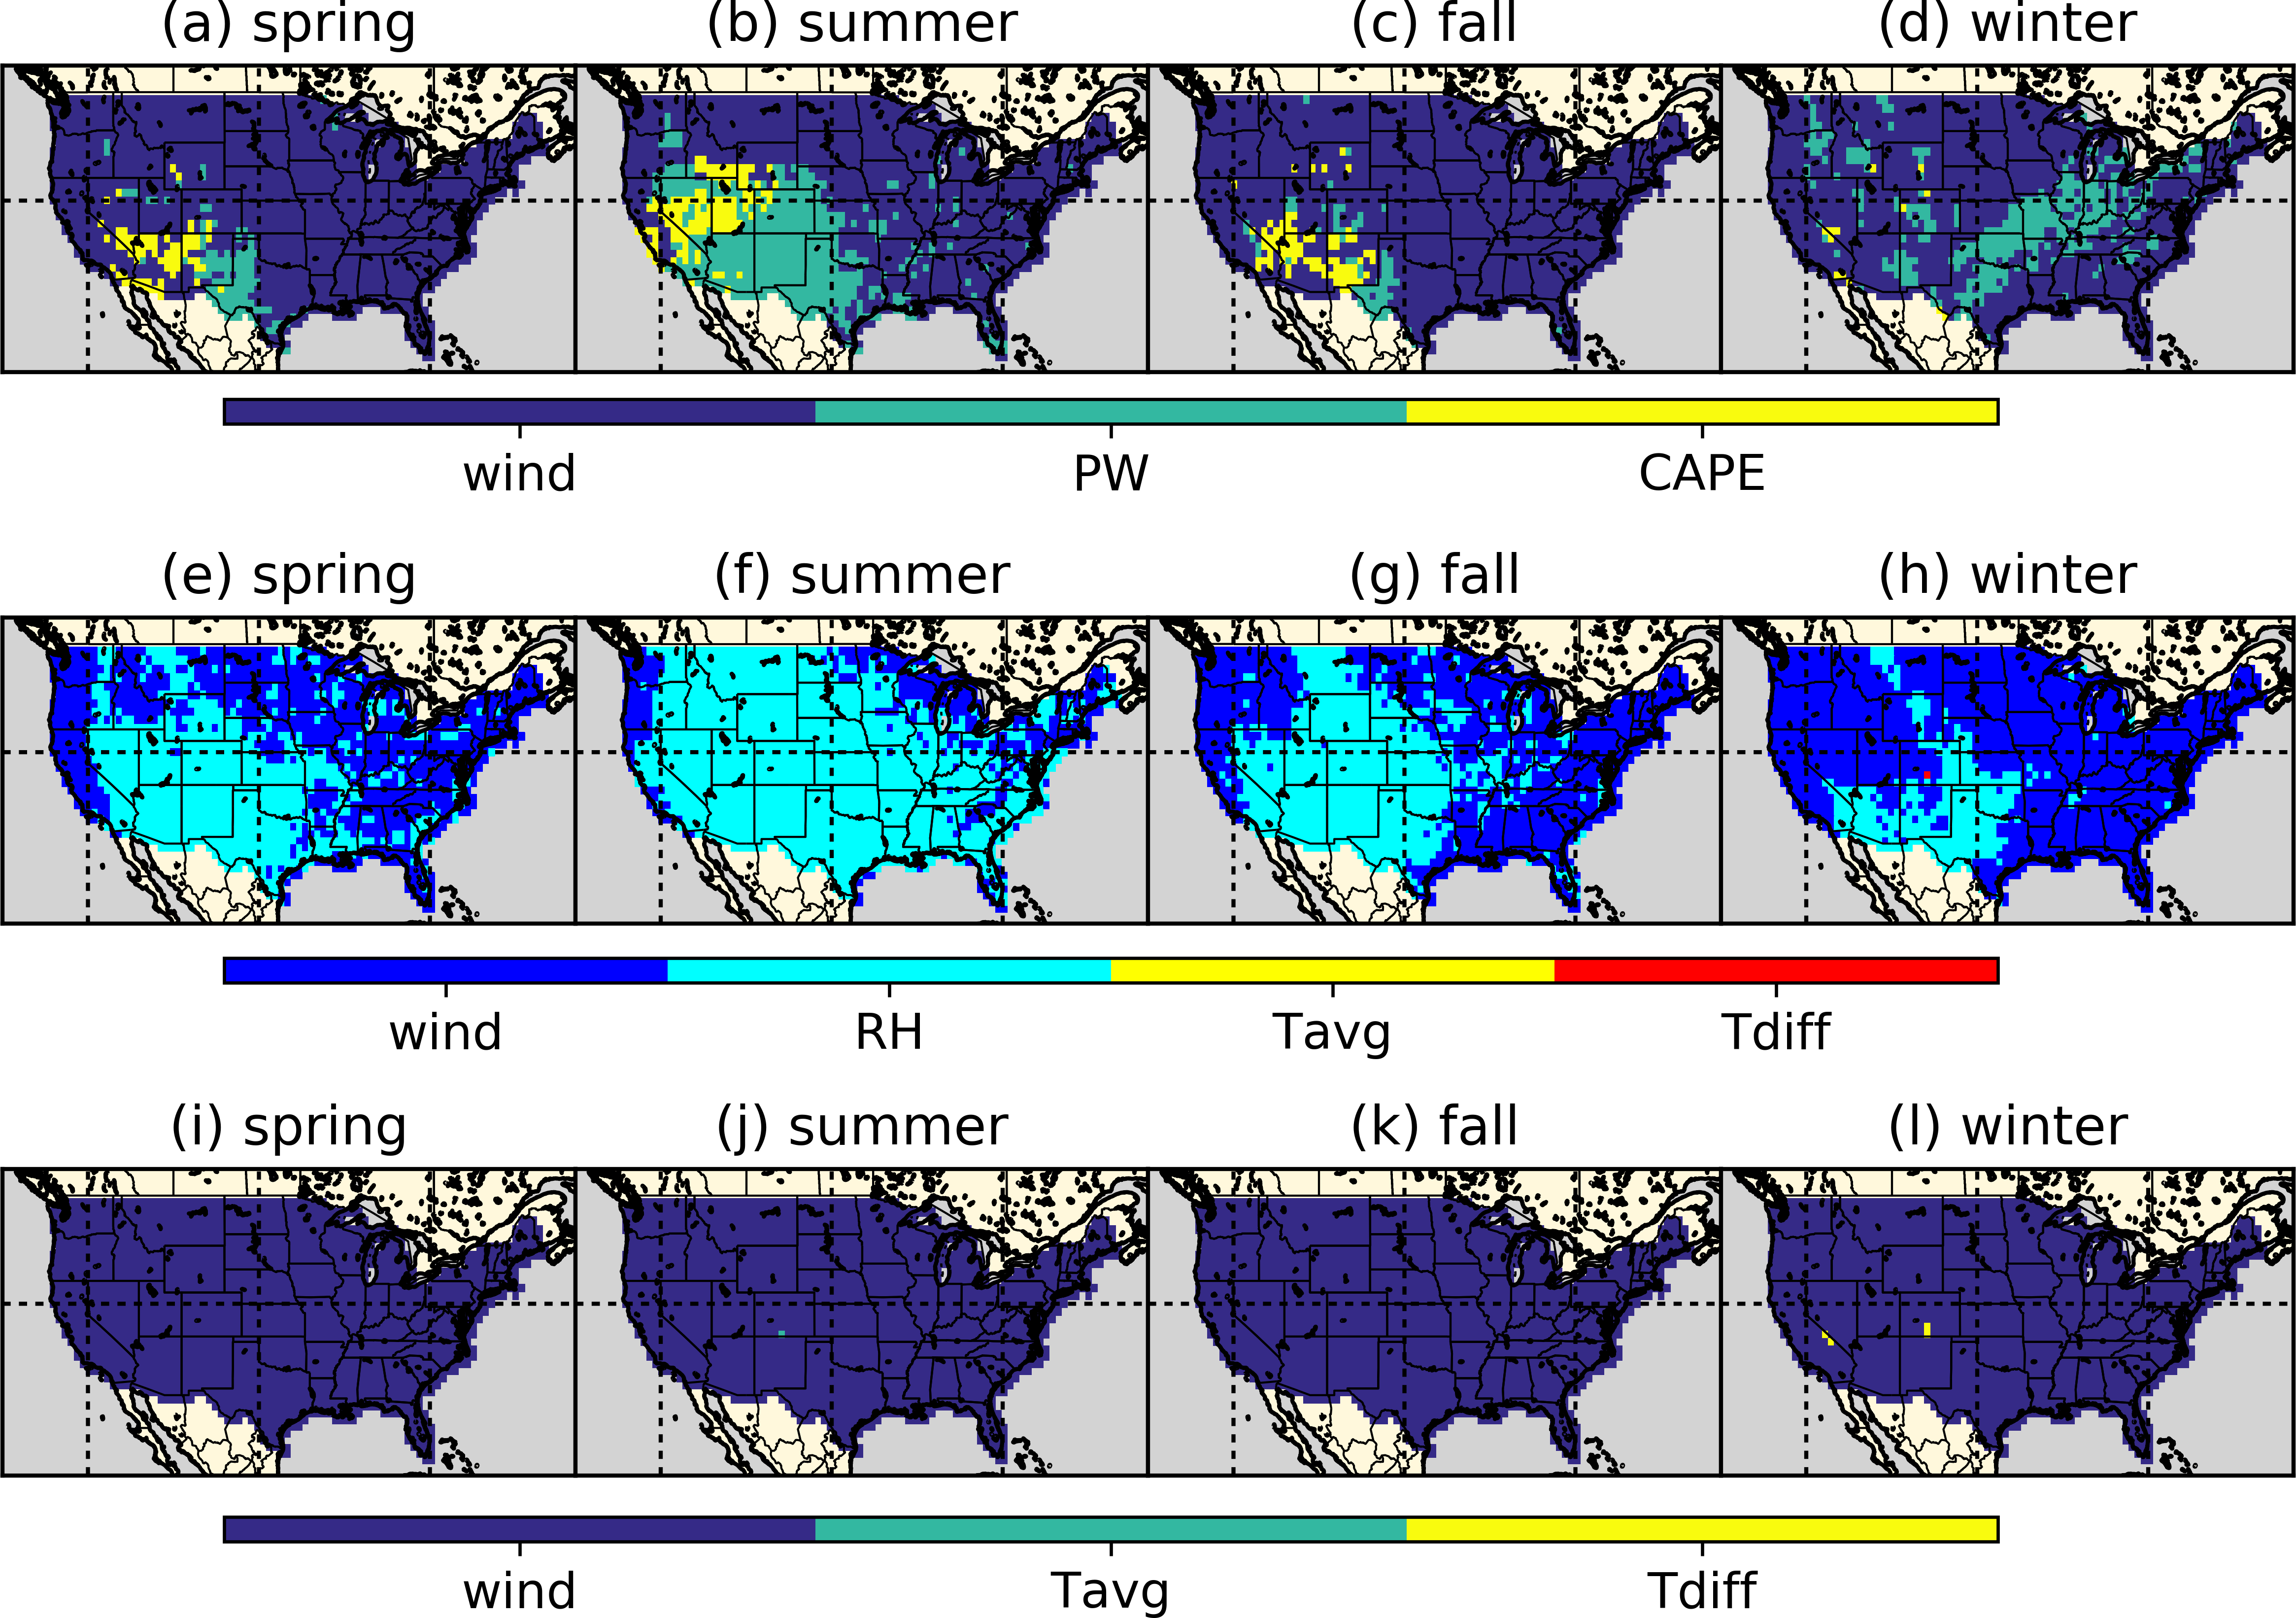
\includegraphics[width=\linewidth]{pics/ch4/figS4.png}
	\caption{Seasonal variations in the dominant controls, from ERA-Interim. Similar to figure \ref{fig:4-6}, but from ERA-Interim data.}
	\label{fig:4-S4}
\end{figure}

\begin{figure}[htbp]
	\centering
	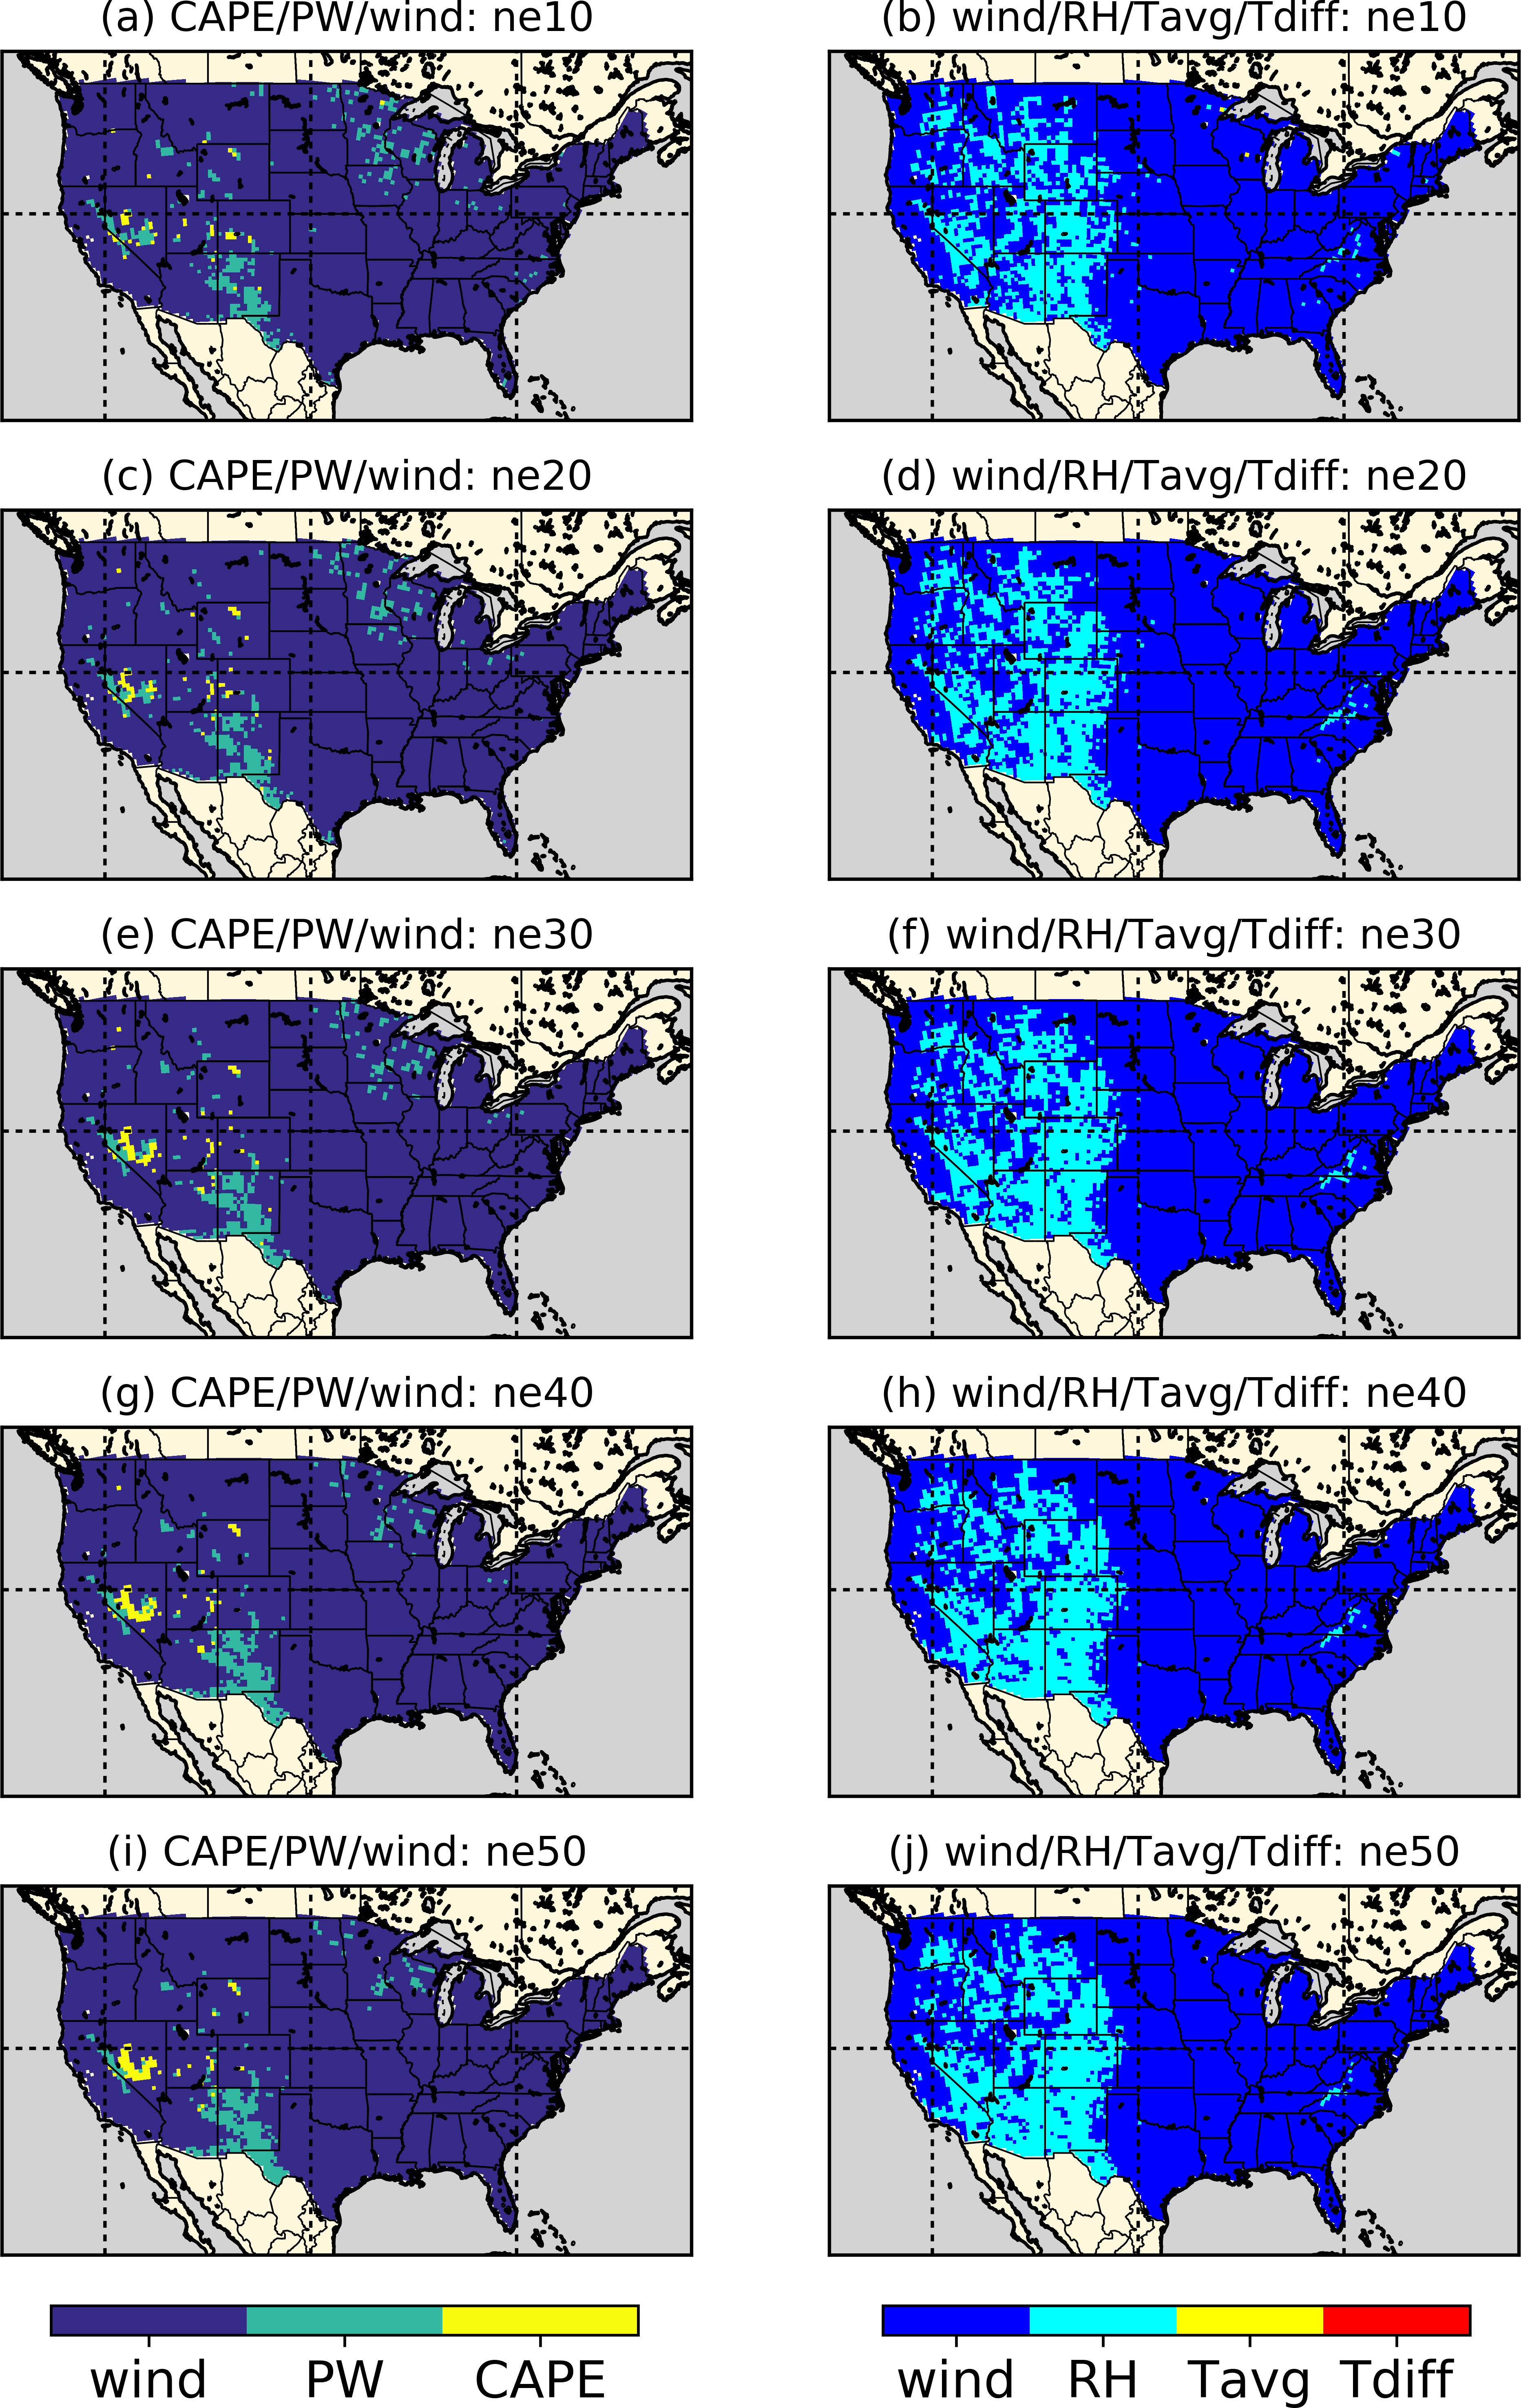
\includegraphics[width=10cm]{pics/ch4/figS5.png}
	\caption{Robustness check of the derived map in figure \ref{fig:4-5}a. Here the number of extreme events used in the analysis (ne) varies between 10 and 50, and the maps share a similar pattern as figure \ref{fig:4-5}a.}
	\label{fig:4-S5}
\end{figure}

\begin{figure}[htbp]
	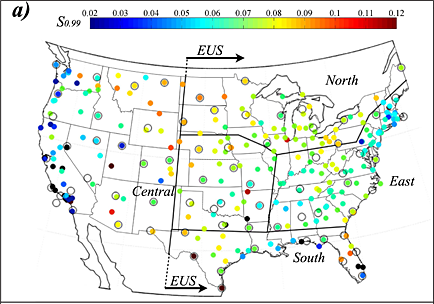
\includegraphics[width=\linewidth]{pics/ch4/figS6.png}
	\caption{Sub-regions division in \textit{Lepore et al.} [2015]. \textcopyright \textit{Lepore et al.} (2015). Used with permission.}
	\label{fig:4-S6}
\end{figure}